
\section{在overleaf上使用模板}
在个人电脑上安装\LaTeX 并不麻烦,但是很多用户可能更希望在网页上使用\LaTeX 。目前使用比较广泛的在线LaTeX编辑器是overleaf,网址为\url{https://www.overleaf.com/}。只需要将模板上传至overleaf,即可在线使用。
具体步骤如下:

\begin{enumerate}
    \item 新建一个project,并将模板压缩成zip文件上传至网站。
    \begin{center}
        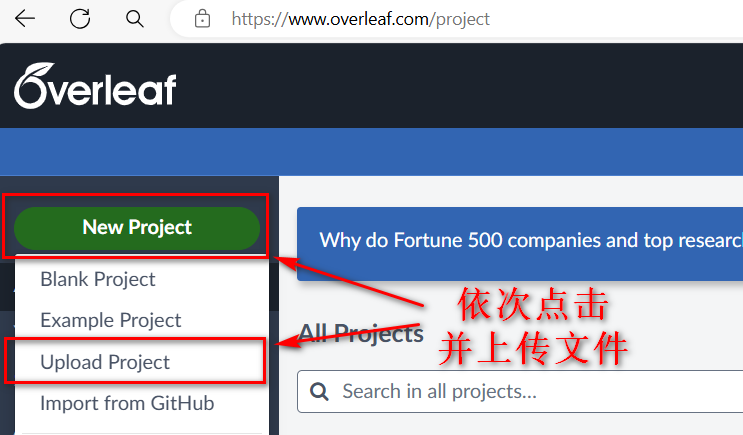
\includegraphics[width=\linewidth]{overleaf_0.png}
    \end{center}

    \item 在Windows系统的电脑上,打开C盘,搜索Fonts,找到该文件夹,然后将里面的simkai.ttf(楷体), simsun.ttf(宋体), times.ttc(Times New Roman), simhei.ttf(黑体),timesbd.ttf(Times New Roman bold)几种字体上传至Project的根目录/主文件夹下。

    如果不执行这一步操作,仍然可以使用,但是需要注意的是,因overleaf的系统为Ubuntu,字体与Windows系统下的字体略有差别。
    
    \item 点击菜单按钮,并将编译方式设置成xeLaTeX.
    \begin{center}
        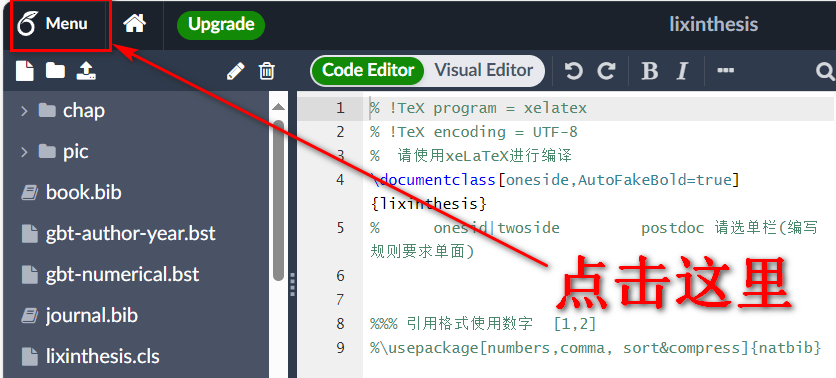
\includegraphics[width=0.65\linewidth]{overleaf_1.png}
        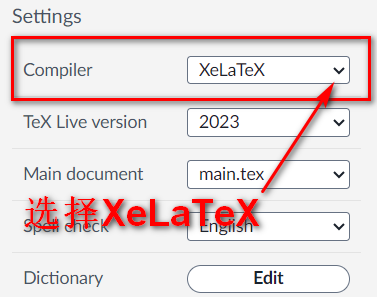
\includegraphics[width=0.3\linewidth]{overleaf_2.png}
    \end{center}
    \item 点击中间编译按钮,编译文件生成PDF文档。
    \begin{center}
        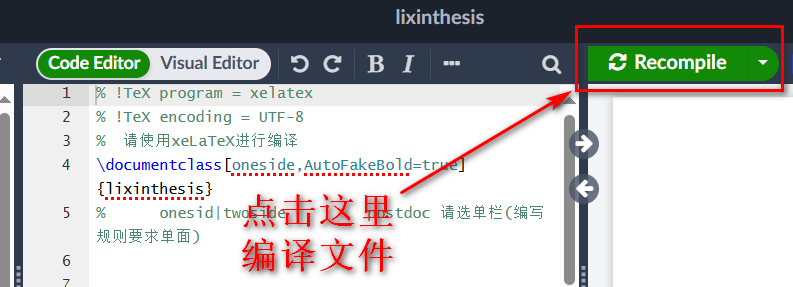
\includegraphics[width=\linewidth]{overleaf_3.png}
    \end{center}
\end{enumerate}

